\documentclass{beamer}

%style
\mode<presentation>
\usetheme{Boadilla}

%Packages
\usepackage[utf8]{inputenc}
\usepackage[ngerman]{babel}
\usepackage{graphicx}
\usepackage{booktabs}
\usepackage{mathtools}
\usepackage{amsmath}
\usepackage{listings}
\usepackage[utf8]{inputenc}
\usepackage[ngerman]{babel}
\usepackage[T1]{fontenc}
\usepackage{lmodern}
\usepackage{tabto}
\usepackage{listings}
\usepackage{framed} 
\usepackage{xcolor} 
\colorlet{shadecolor}{gray!25}
%bibtex
\usepackage[backend=biber, style=authoryear]{biblatex}
\addbibresource{referenzen.bib}

%Einstellungen der Präsentation
\title[Cybersecurity]{Flubot:\\ Android-Malware verbreitet sich über Fake-Patches\\!WIP!}
\author{Moritz Rupp}
\institute[MR]{Hochschule Albstadt-Sigmaringen}
\setbeamertemplate{navigation symbols}{}%remove navigation symbols
\date{tobedated - WS 21/22}

%Beginn der Präsentation
\begin{document}

%Titelseite
\begin{frame}
\titlepage
\end{frame}

\begin{frame}{Leitartikel}
\begin{center}
 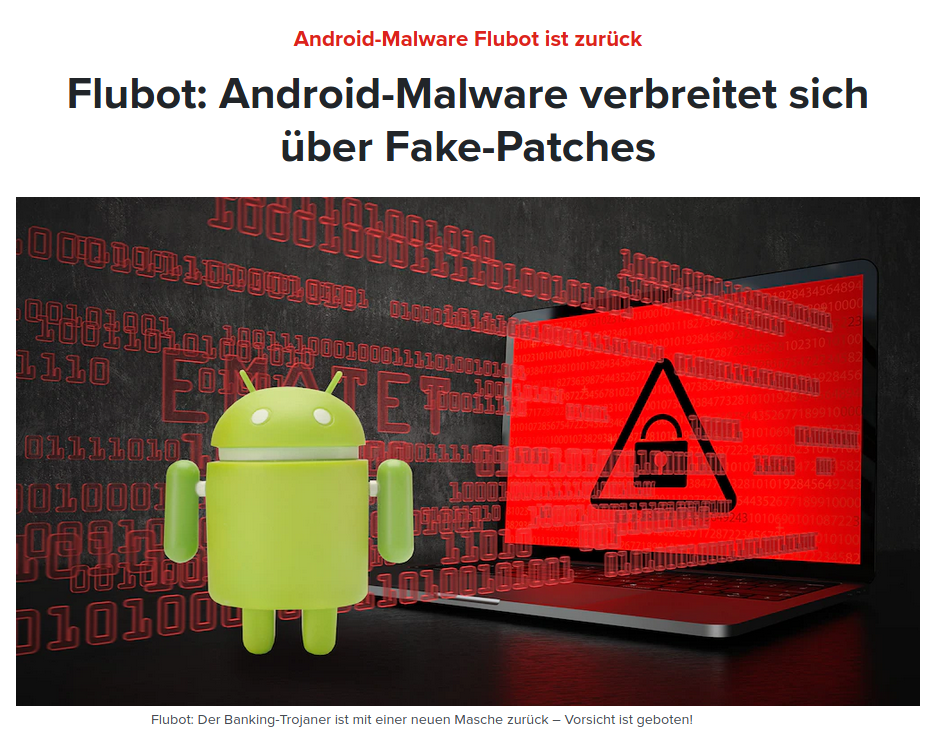
\includegraphics[scale=0.31]{bild.png} 

\end{center}

\end{frame}
%Inhaltsverzeichnis
\begin{frame}
\frametitle{Inhalt}
\tableofcontents    
\end{frame}
\section{Terminologie}
\begin{frame}{Terminologie}
\begin{block}{Malware}
Software zu ausführung unerwünschter bzw. schädlicher Funktionen.
\end{block}
\begin{block}{Banking Trojaner}
 Vermeintlich harmlose Anwendung dringt in System ein und greift Daten ab. $\Rightarrow$ Banking Login Daten.
\end{block}
\begin{block}{Phishing}
Vortäuschung von Diensten zu erlangung von Login Informationen.
\end{block}

\begin{block}{Botnetze}
 Große Anzahl an Geräten(Bots) die über Netzwerke automatisiert Malware betreiben.
\end{block}

\end{frame}
\section{Was ist Flubot?}
\begin{frame}{Was ist Flubot?}
\begin{itemize}
 \item Android Malware
 \item Banking Trojaner
 \item Verbreitung über SMS Nachrichten
 \item Nutzung von Botnetzten und Phishing Methoden
 \item Nach wie vor im Umlauf
\end{itemize}

\end{frame}
\begin{frame}{Trivia}
 \section{Trivia}
 \begin{itemize}
 
  \item Erstes Auftreten Ende 2020 in Spanien\\
  	- Frühjar 2021 in Deutschland
  \item Weltweite Verbreitung im laufe des Jahres 2021
  \item \raisebox{-0.9ex}{\~{}}13 Millionen Infizierte Geräte
  \item Finanzieller Schaden schwer festellbar \raisebox{-0.9ex}{\~{}} 8 stelligem Bereich!
 \end{itemize}
\end{frame}

\section{Funktionsweiße}
\begin{frame}{Funktionsweiße}
\begin{itemize}
 \item Opfer erhält eine SMS mitsamt Link.
 \item Der Link führt zu einer Webseite auf der ein APK Download bereit steht.
 \item Durch Download der APK wird das betroffene Gerät infiziert.
 \item Die Malware durchsucht nun die Kontaktliste und schickt über diese weitere Phishing Nachrichten!
 \item Nun werden über ausgewählte Apps Phishing Overlays gelegt\\
 $\Rightarrow$ Jegliche Eingaben werden nun an Angreifer weitergeleitet
\end{itemize}
\end{frame}
\subsection{Verbreitung}
\begin{frame}{Verbreitung}
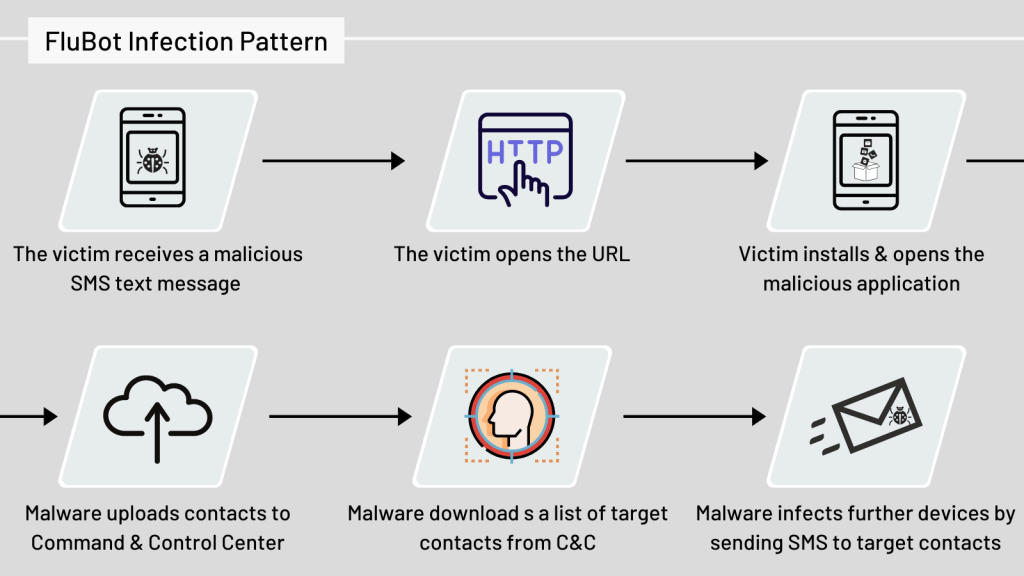
\includegraphics[scale=0.41]{command_control_server.png}
\end{frame}

\begin{frame}{Phishing Methoden}
\begin{itemize}
 \item Anfangs wird eine vermeintliche Voicemail als Köder verwendet
 \item Seit Frühjahr 2021 vermehrt Packerlieferdienste
 \item Ab mitte 2021 'Fake security patches' gegen Flubot selbst
 \item Anfang 2022 nun Adobe Apps
 \item Flubot variert und wechselt häufig Phishing Köder! 
\end{itemize}


\end{frame}
\begin{frame}
\begin{center}
 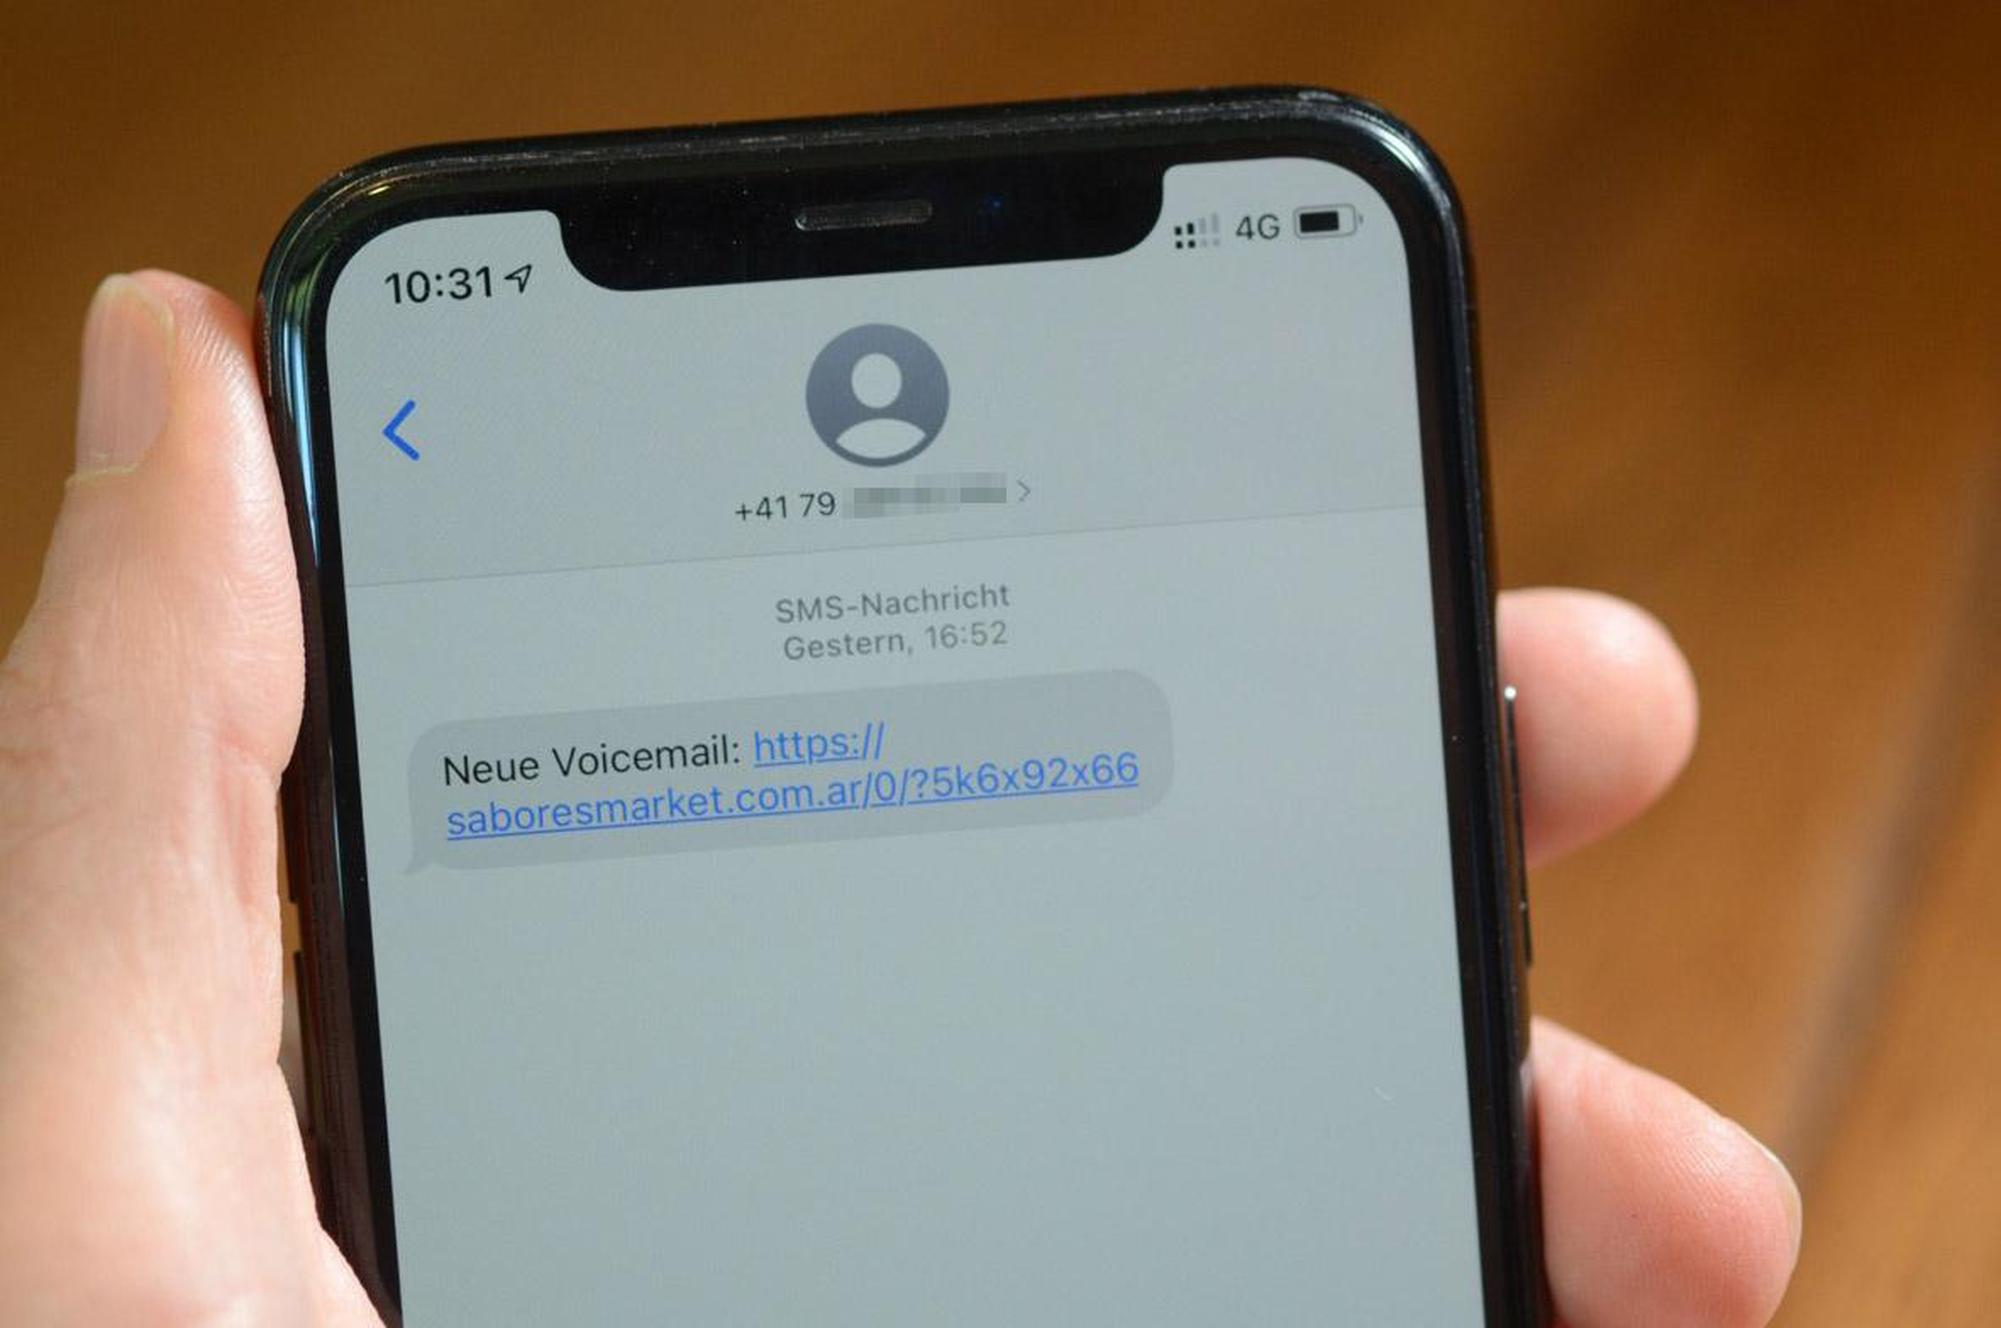
\includegraphics[scale=0.15]{firstvoice.jpg}

\end{center}


\end{frame}


\begin{frame}
\begin{center}
 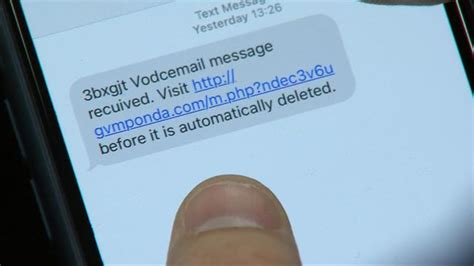
\includegraphics[scale=0.51]{voice.jpeg}

\end{center}
\end{frame}
\begin{frame}
\begin{center}
 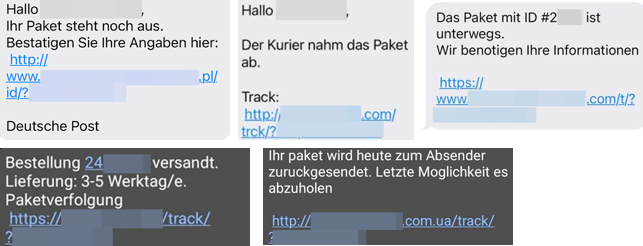
\includegraphics[scale=0.51]{external-content.duckduckgo.com.png}

\end{center}


\end{frame}
\begin{frame}
\begin{center}
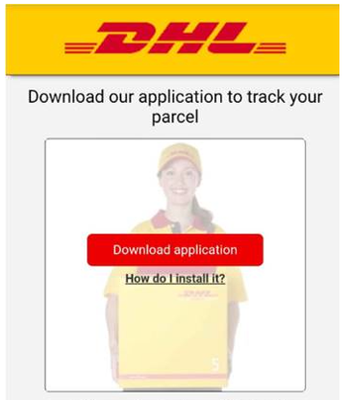
\includegraphics[scale=0.51]{dhl.png}

\end{center}


\end{frame}
\subsection{Post-Infection}
\begin{frame}{Post-Infection}
 \begin{itemize}
  \item Verbindungsaufbau zum Command and Control Server
 \end{itemize}

\begin{block}{Command and Control Server}
Hauptzentrale des Botnetzes! Hier wird die Malware gesteuert!
\end{block}
\begin{itemize}
 \item Gerät schickt alle Kontakte und installierten Apps an den C\&C Server!
\item Dieser antwortet mit einer neuen Liste neuer Kontakte\\
$\Rightarrow$ Über diese werden weitere Phishing SMS versendet!
\item Zudem wird eine Liste der geziehlten Anwendungen geschickt
\item Über diese Anwendungen wird nun das eigentliche Phishing Overlay gelegt!
 \end{itemize}

\end{frame}
\begin{frame}
\begin{center}
 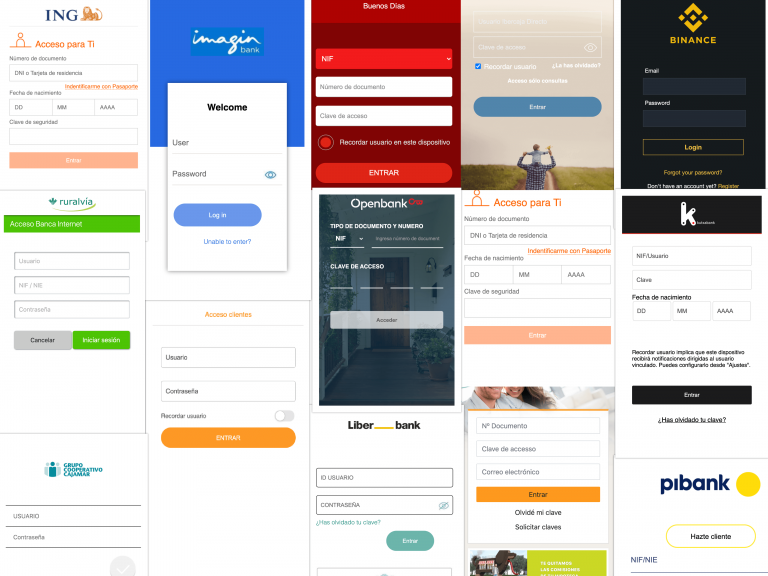
\includegraphics[scale=0.51]{infected.png}

\end{center}


\end{frame}
\section{Technische Analyse}
\begin{frame}{Technische Analyse}
\begin{itemize}
 \item Die Malware APK ist komplett in Java geschrieben
 \item Läuft ab Android Version 4.1.2
 \item Wird stetig weiterentwickelt
 \item Verwendung von String Obfuscation um Reverse Engineering zu erschweren!
 \item Über 30 Kommandos für Kommunikation zwischen Gerät und C\&C möglich!
\end{itemize}
\end{frame}
\begin{frame}{Command and control Server}
 
\end{frame}

\begin{frame}
\begin{shaded}
\#Kommandos von dem C\&C Server an das Gerät

GET\_CONTACTS - Schicke Kontakte an den Server.\\
RETRY\_INJECT - Versuche erneut die Anwendung zu infizieren\\
BLOCK - Jegliche Kommunikation blocken\\
UNINSTALL\_APP - Deinstalltion der Malware\\
SEND\_SMS - Versenden von SMS\\
DISABLE\_PLAY\_PROTECT - Den Virenschutz des Google Play stores deaktivieren\footnote{https://raw.githubusercontent.com/prodaft/malware-ioc/master/FluBot/FluBot.pdf}
\end{shaded}
\end{frame}

\begin{frame}{Netzwerkstrukur}
- Flubot verwendet gekapperte Webeiten als Hosts.\\
- Über 200 betroffene Blogs!\\
- Keine Feste Domain oder IP!\\
- Domaingenerierung anhand des DGA\\
- Auflösung über DNS über HTTPS\\
- Nutzt Services wie dns.google
\end{frame}
\begin{frame}
\begin{center}
 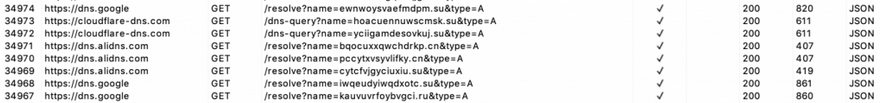
\includegraphics[scale=0.51]{dns.png}

\end{center}
\end{frame}
\section{Conclusion}
\begin{frame}{Conclusion}
 - Pishing nach wie vor größte Bedrohungslage\\
 - Keine technische Lösung!\\
 - Geringer schutz durch 2FA möglich!\\
 - Nachhaltiger Schutz bzw. Bekämpfung nur durch bessere Aufklärung und Bildung möglich!
\end{frame}
\section{Quellen}
\begin{frame}{Quellen}
https://de.statista.com/statistik/daten/studie/1235321\\
https://de.statista.com/themen/1355/android/\\
https://www.telekom.com/en/blog/group/article/flubot-under-the-microscope-636368\\
https://www.telekom.com/en/blog/group/article/flubot-under-the-microscope-636368\\
https://www.computerbild.de/artikel/cb-News-Sicherheit-Flubot-Gefaehrliche-Android-Malware-verbreitet-sich-ueber-Fake-Patches-30863335.html\\
https://computerwelt.at/news/android-malware-flubot-stuermt-top-ten\\
https://www.telekom.com/en/blog/group/article/flubot-under-the-microscope-636368\\

\end{frame}

\end{document}
